\documentclass[11pt]{article}
\usepackage{amsmath,amssymb,amsfonts,amsthm,complexity,graphicx}
%%%%%%%%%%%%%%%%%%%%%%%%%%%%%%%%%%%%%%%%%%%%%%%%%%%%%%
%
% This file should be called  preamble.tex 
% Your main LaTeX file should look like :
%
%	\documentclass[11pt]{article}
%	\usepackage{amsmath,amssymb,amsfonts,amsthm,complexity}
%
%	%%%%%%%%%%%%%%%%%%%%%%%%%%%%%%%%%%%%%%%%%%%%%%%%%%%%%%
%
% This file should be called  preamble.tex 
% Your main LaTeX file should look like :
%
%	\documentclass[11pt]{article}
%	\usepackage{amsmath,amssymb,amsfonts,amsthm,complexity}
%
%	%%%%%%%%%%%%%%%%%%%%%%%%%%%%%%%%%%%%%%%%%%%%%%%%%%%%%%
%
% This file should be called  preamble.tex 
% Your main LaTeX file should look like :
%
%	\documentclass[11pt]{article}
%	\usepackage{amsmath,amssymb,amsfonts,amsthm,complexity}
%
%	\input{preamble.tex}
%	\begin{document}
%
%	\lecture{LECTURE NO.}{TITLE OF SCRIBE}{DATE}{Jayalal Sarma M.N.}{YOUR NAME}
%	\theme{THEME FOCUS}
%	\lectureplan{A BRIEF DESCRIPTION OF THE LECTURE}
%	
%	\section{TOPIC 1}
%	...
%	\section{TOPIC 2}
% 	...
%	\end{document}
% If there is not title, leave it as {}
 

\newtheorem{theorem}{Theorem}
\newtheorem{corollary}[theorem]{Corollary}
\newtheorem{lemma}[theorem]{Lemma}
\newtheorem{observation}[theorem]{Observation}
\newtheorem{proposition}[theorem]{Proposition}
\newtheorem{claim}[theorem]{Claim}
\newtheorem{fact}[theorem]{Fact}
\newtheorem{example}[theorem]{Example}
\newtheorem{assumption}[theorem]{Assumption}

\theoremstyle{definition}
\newtheorem{definition}[theorem]{Definition}

\theoremstyle{remark}
\newtheorem{remark}[theorem]{Remark}

% Setting theorem style back for theorems defined in main file.
\theoremstyle{plain}

%\newenvironment{proof}{\noindent{\bf Proof}\hspace*{1em}}{\qed\bigskip}
\newenvironment{proof-sketch}{\noindent{\bf Sketch of Proof}\hspace*{1em}}{\qed\bigskip}
\newenvironment{proof-idea}{\noindent{\bf Proof Idea}\hspace*{1em}}{\qed\bigskip}
\newenvironment{proof-of-lemma}[1]{\noindent{\bf Proof of Lemma #1}\hspace*{1em}}{\qed\bigskip}
\newenvironment{proof-attempt}{\noindent{\bf Proof Attempt}\hspace*{1em}}{\qed\bigskip}
\newenvironment{proofof}[1]{\noindent{\bf Proof}
of #1:\hspace*{1em}}{\qed\bigskip}

%%%%%%%%%%%%%%%%%%%%%%%%%%%%%%%%%%%%%%%%%%%%%%%%%%%
% Useful Complexity Classes
%%%%%%%%%%%%%%%%%%%%%%%%%%%%%%%%%%%%%%%%%%%%%%%%%%%
\newcommand{\ntime}{\hbox{NTIME}}
\newcommand{\nspace}{\hbox{NSPACE}}
\newcommand{\conspace}{\hbox{co-NSPACE}}
\newcommand{\np}{\hbox{NP}}
\newcommand{\pspace}{\hbox{PSPACE}}
\newcommand{\lspace}{\hbox{L}}
\newcommand{\conp}{\hbox{coNP}}
\newcommand{\exptime}{\hbox{EXPTIME}}
\newcommand{\elem}{\hbox{E}}
\newcommand{\nl}{\hbox{NL}}
\newcommand{\bpp}{\hbox{BPP}}
\newcommand{\nregexp}{\hbox{NREGEXP}}
\newcommand{\tqbf}{\hbox{TQBF}}
\newcommand{\threesat}{\hbox{3SAT}}
\newcommand{\cvp}{\hbox{CVP}}
\newcommand{\stconn}{\hbox{STCONN}}
\newcommand{\ispath}{\hbox{ISPATH}}

%\newcommand{\class}{\hbox{$\mathbb{C}$}} 
%\newcommand{\class}{\hbox{$\mathbf{C}$}} 

\newcommand{\lep}{\leq _{\hbox{P}}}
\newcommand{\lel}{\leq _{\hbox{L}}}
\newcommand{\aspace}[1]{{\rm ASPACE}(#1)}
\newcommand{\atime}[1]{{\rm ATIME}(#1)}
\newcommand{\dtime}[1]{{\rm DTIME}(#1)}
\newcommand{\spa}[1]{{\rm SPACE}(#1)}
\newcommand{\ti}[1]{{\rm TIME}(#1)}
\newcommand{\ap}{{\rm AP}}
\newcommand{\al}{{\rm AL}}


%%%%%%%%%%%%%%%%%%%%%%%%%%%%%%%%%%%%%%%%%%%%%%%%%%%
% Useful Macros
%%%%%%%%%%%%%%%%%%%%%%%%%%%%%%%%%%%%%%%%%%%%%%%%%%%
\renewcommand{\Pr}[1]{\mathify{\mbox{Pr}\left[#1\right]}}
\newcommand{\Exp}[1]{\mathify{\mbox{Exp}\left[#1\right]}}
\newcommand{\bigO}O
\newcommand{\set}[1]{\mathify{\left\{ #1 \right\}}}
\def\half{\frac{1}{2}}

\def\implies{\Rightarrow}
\def\prob#1#2{{\mathop{{\rm Prob}}_{#1}}\left[#2 \right]}
\def\var#1#2{{\mathop{{\rm Var}}_{#1}}[#2]}
\def\expec#1#2{{\mathop{{\rm E}}_{#1}}[#2]}
\def\sizeof#1{\left| #1\right|}
\def\setof#1{\left\{ #1\right\}  }

\newcommand{\F}{{\mathbb{F}}}
\newcommand{\Z}{{\mathbb{Z}}}
%\newcommand{\qed}{\rule{7pt}{7pt}}

% \makeatletter
% \@addtoreset{figure}{section}
% \@addtoreset{table}{section}
% \@addtoreset{equation}{section}
% \makeatother

\newcommand{\FOR}{{\bf for}}
\newcommand{\TO}{{\bf to}}
\newcommand{\DO}{{\bf do}}
\newcommand{\WHILE}{{\bf while}}
\newcommand{\AND}{{\bf and}}
\newcommand{\IF}{{\bf if}}
\newcommand{\THEN}{{\bf then}}
\newcommand{\ELSE}{{\bf else}}
\newcommand{\N}{\mathbb{N}}

% \renewcommand{\thefigure}{\thesection.\arabic{figure}}
% \renewcommand{\thetable}{\thesection.\arabic{table}}
% \renewcommand{\theequation}{\thesection.\arabic{equation}}

% Calligraphic letters
\newcommand{\calA}{{\cal A}}
\newcommand{\calB}{{\cal B}}
\newcommand{\calC}{{\cal C}}
\newcommand{\calD}{{\cal D}}
\newcommand{\calE}{{\cal E}}
\newcommand{\calF}{{\cal F}}
\newcommand{\calG}{{\cal G}}
\newcommand{\calH}{{\cal H}}
\newcommand{\calI}{{\cal I}}
\newcommand{\calJ}{{\cal J}}
\newcommand{\calK}{{\cal K}}
\newcommand{\calL}{{\cal L}}
\newcommand{\calM}{{\cal M}}
\newcommand{\calN}{{\cal N}}
\newcommand{\calO}{{\cal O}}
\newcommand{\calP}{{\cal P}}
\newcommand{\calQ}{{\cal Q}}
\newcommand{\calR}{{\cal R}}
\newcommand{\calS}{{\cal S}}
\newcommand{\calT}{{\cal T}}
\newcommand{\calU}{{\cal U}}
\newcommand{\calV}{{\cal V}}
\newcommand{\calW}{{\cal W}}
\newcommand{\calX}{{\cal X}}
\newcommand{\calY}{{\cal Y}}
\newcommand{\calZ}{{\cal Z}}


% Some macro's from Speilman's course.

\makeatletter
\def\fnum@figure{{\bf Figure \thefigure}}
\def\fnum@table{{\bf Table \thetable}}
\long\def\@mycaption#1[#2]#3{\addcontentsline{\csname
  ext@#1\endcsname}{#1}{\protect\numberline{\csname 
  the#1\endcsname}{\ignorespaces #2}}\par
  \begingroup
    \@parboxrestore
    \small
    \@makecaption{\csname fnum@#1\endcsname}{\ignorespaces #3}\par
  \endgroup}
\def\mycaption{\refstepcounter\@captype \@dblarg{\@mycaption\@captype}}
\makeatother

\newcommand{\figcaption}[1]{\mycaption[]{#1}}
\newcommand{\tabcaption}[1]{\mycaption[]{#1}}


%%%%%%%%%%%%%%%%%%%%%%%%%%%%%%%%%%%%%%%%%%%%%%%%%%%%%%%%%%%%%%%%%%%%%%
% Feel free to ignore the rest of this file.

%%%%%%%%%%%%%%%%%%%%%%%%%%%%%%%
% Margins and page indentations
% DO NOT EDIT
%%%%%%%%%%%%%%%%%%%%%%%%%%%%%%
\textwidth=6in
\oddsidemargin=0.25in
\evensidemargin=0.25in
\topmargin=-0.1in
\footskip=0.8in
\parindent=0.0cm
\parskip=0.3cm
\textheight=8.00in
\setcounter{tocdepth} {3}
\setcounter{secnumdepth} {2}
\sloppy


\newcommand{\handout}[5]{
   \renewcommand{\thepage}{#1-\arabic{page}}
   \noindent
   \begin{center}
   \framebox{
      \vbox{
    \hbox to 5.78in { {\bf CS6840: Advanced Complexity Theory} \hfill #2 }
       \vspace{4mm}
       \hbox to 5.78in { {\Large \hfill #5  \hfill} }
       \vspace{2mm}
       \hbox to 5.78in { {\em #3 \hfill #4} }
      }
   }
   \end{center}
   \vspace*{4mm}
}

\newcommand{\lecture}[5]{\handout{#1}{#3}{Lecturer:~#4}{Scribe: #5}{Lecture~#1~: #2}}

\newcommand{\lectureplan}[1]{{\sc Lecture Plan:}#1\\}
\newcommand{\theme}[1]{{\sc Theme:} #1\\}

%	\begin{document}
%
%	\lecture{LECTURE NO.}{TITLE OF SCRIBE}{DATE}{Jayalal Sarma M.N.}{YOUR NAME}
%	\theme{THEME FOCUS}
%	\lectureplan{A BRIEF DESCRIPTION OF THE LECTURE}
%	
%	\section{TOPIC 1}
%	...
%	\section{TOPIC 2}
% 	...
%	\end{document}
% If there is not title, leave it as {}
 

\newtheorem{theorem}{Theorem}
\newtheorem{corollary}[theorem]{Corollary}
\newtheorem{lemma}[theorem]{Lemma}
\newtheorem{observation}[theorem]{Observation}
\newtheorem{proposition}[theorem]{Proposition}
\newtheorem{claim}[theorem]{Claim}
\newtheorem{fact}[theorem]{Fact}
\newtheorem{example}[theorem]{Example}
\newtheorem{assumption}[theorem]{Assumption}

\theoremstyle{definition}
\newtheorem{definition}[theorem]{Definition}

\theoremstyle{remark}
\newtheorem{remark}[theorem]{Remark}

% Setting theorem style back for theorems defined in main file.
\theoremstyle{plain}

%\newenvironment{proof}{\noindent{\bf Proof}\hspace*{1em}}{\qed\bigskip}
\newenvironment{proof-sketch}{\noindent{\bf Sketch of Proof}\hspace*{1em}}{\qed\bigskip}
\newenvironment{proof-idea}{\noindent{\bf Proof Idea}\hspace*{1em}}{\qed\bigskip}
\newenvironment{proof-of-lemma}[1]{\noindent{\bf Proof of Lemma #1}\hspace*{1em}}{\qed\bigskip}
\newenvironment{proof-attempt}{\noindent{\bf Proof Attempt}\hspace*{1em}}{\qed\bigskip}
\newenvironment{proofof}[1]{\noindent{\bf Proof}
of #1:\hspace*{1em}}{\qed\bigskip}

%%%%%%%%%%%%%%%%%%%%%%%%%%%%%%%%%%%%%%%%%%%%%%%%%%%
% Useful Complexity Classes
%%%%%%%%%%%%%%%%%%%%%%%%%%%%%%%%%%%%%%%%%%%%%%%%%%%
\newcommand{\ntime}{\hbox{NTIME}}
\newcommand{\nspace}{\hbox{NSPACE}}
\newcommand{\conspace}{\hbox{co-NSPACE}}
\newcommand{\np}{\hbox{NP}}
\newcommand{\pspace}{\hbox{PSPACE}}
\newcommand{\lspace}{\hbox{L}}
\newcommand{\conp}{\hbox{coNP}}
\newcommand{\exptime}{\hbox{EXPTIME}}
\newcommand{\elem}{\hbox{E}}
\newcommand{\nl}{\hbox{NL}}
\newcommand{\bpp}{\hbox{BPP}}
\newcommand{\nregexp}{\hbox{NREGEXP}}
\newcommand{\tqbf}{\hbox{TQBF}}
\newcommand{\threesat}{\hbox{3SAT}}
\newcommand{\cvp}{\hbox{CVP}}
\newcommand{\stconn}{\hbox{STCONN}}
\newcommand{\ispath}{\hbox{ISPATH}}

%\newcommand{\class}{\hbox{$\mathbb{C}$}} 
%\newcommand{\class}{\hbox{$\mathbf{C}$}} 

\newcommand{\lep}{\leq _{\hbox{P}}}
\newcommand{\lel}{\leq _{\hbox{L}}}
\newcommand{\aspace}[1]{{\rm ASPACE}(#1)}
\newcommand{\atime}[1]{{\rm ATIME}(#1)}
\newcommand{\dtime}[1]{{\rm DTIME}(#1)}
\newcommand{\spa}[1]{{\rm SPACE}(#1)}
\newcommand{\ti}[1]{{\rm TIME}(#1)}
\newcommand{\ap}{{\rm AP}}
\newcommand{\al}{{\rm AL}}


%%%%%%%%%%%%%%%%%%%%%%%%%%%%%%%%%%%%%%%%%%%%%%%%%%%
% Useful Macros
%%%%%%%%%%%%%%%%%%%%%%%%%%%%%%%%%%%%%%%%%%%%%%%%%%%
\renewcommand{\Pr}[1]{\mathify{\mbox{Pr}\left[#1\right]}}
\newcommand{\Exp}[1]{\mathify{\mbox{Exp}\left[#1\right]}}
\newcommand{\bigO}O
\newcommand{\set}[1]{\mathify{\left\{ #1 \right\}}}
\def\half{\frac{1}{2}}

\def\implies{\Rightarrow}
\def\prob#1#2{{\mathop{{\rm Prob}}_{#1}}\left[#2 \right]}
\def\var#1#2{{\mathop{{\rm Var}}_{#1}}[#2]}
\def\expec#1#2{{\mathop{{\rm E}}_{#1}}[#2]}
\def\sizeof#1{\left| #1\right|}
\def\setof#1{\left\{ #1\right\}  }

\newcommand{\F}{{\mathbb{F}}}
\newcommand{\Z}{{\mathbb{Z}}}
%\newcommand{\qed}{\rule{7pt}{7pt}}

% \makeatletter
% \@addtoreset{figure}{section}
% \@addtoreset{table}{section}
% \@addtoreset{equation}{section}
% \makeatother

\newcommand{\FOR}{{\bf for}}
\newcommand{\TO}{{\bf to}}
\newcommand{\DO}{{\bf do}}
\newcommand{\WHILE}{{\bf while}}
\newcommand{\AND}{{\bf and}}
\newcommand{\IF}{{\bf if}}
\newcommand{\THEN}{{\bf then}}
\newcommand{\ELSE}{{\bf else}}
\newcommand{\N}{\mathbb{N}}

% \renewcommand{\thefigure}{\thesection.\arabic{figure}}
% \renewcommand{\thetable}{\thesection.\arabic{table}}
% \renewcommand{\theequation}{\thesection.\arabic{equation}}

% Calligraphic letters
\newcommand{\calA}{{\cal A}}
\newcommand{\calB}{{\cal B}}
\newcommand{\calC}{{\cal C}}
\newcommand{\calD}{{\cal D}}
\newcommand{\calE}{{\cal E}}
\newcommand{\calF}{{\cal F}}
\newcommand{\calG}{{\cal G}}
\newcommand{\calH}{{\cal H}}
\newcommand{\calI}{{\cal I}}
\newcommand{\calJ}{{\cal J}}
\newcommand{\calK}{{\cal K}}
\newcommand{\calL}{{\cal L}}
\newcommand{\calM}{{\cal M}}
\newcommand{\calN}{{\cal N}}
\newcommand{\calO}{{\cal O}}
\newcommand{\calP}{{\cal P}}
\newcommand{\calQ}{{\cal Q}}
\newcommand{\calR}{{\cal R}}
\newcommand{\calS}{{\cal S}}
\newcommand{\calT}{{\cal T}}
\newcommand{\calU}{{\cal U}}
\newcommand{\calV}{{\cal V}}
\newcommand{\calW}{{\cal W}}
\newcommand{\calX}{{\cal X}}
\newcommand{\calY}{{\cal Y}}
\newcommand{\calZ}{{\cal Z}}


% Some macro's from Speilman's course.

\makeatletter
\def\fnum@figure{{\bf Figure \thefigure}}
\def\fnum@table{{\bf Table \thetable}}
\long\def\@mycaption#1[#2]#3{\addcontentsline{\csname
  ext@#1\endcsname}{#1}{\protect\numberline{\csname 
  the#1\endcsname}{\ignorespaces #2}}\par
  \begingroup
    \@parboxrestore
    \small
    \@makecaption{\csname fnum@#1\endcsname}{\ignorespaces #3}\par
  \endgroup}
\def\mycaption{\refstepcounter\@captype \@dblarg{\@mycaption\@captype}}
\makeatother

\newcommand{\figcaption}[1]{\mycaption[]{#1}}
\newcommand{\tabcaption}[1]{\mycaption[]{#1}}


%%%%%%%%%%%%%%%%%%%%%%%%%%%%%%%%%%%%%%%%%%%%%%%%%%%%%%%%%%%%%%%%%%%%%%
% Feel free to ignore the rest of this file.

%%%%%%%%%%%%%%%%%%%%%%%%%%%%%%%
% Margins and page indentations
% DO NOT EDIT
%%%%%%%%%%%%%%%%%%%%%%%%%%%%%%
\textwidth=6in
\oddsidemargin=0.25in
\evensidemargin=0.25in
\topmargin=-0.1in
\footskip=0.8in
\parindent=0.0cm
\parskip=0.3cm
\textheight=8.00in
\setcounter{tocdepth} {3}
\setcounter{secnumdepth} {2}
\sloppy


\newcommand{\handout}[5]{
   \renewcommand{\thepage}{#1-\arabic{page}}
   \noindent
   \begin{center}
   \framebox{
      \vbox{
    \hbox to 5.78in { {\bf CS6840: Advanced Complexity Theory} \hfill #2 }
       \vspace{4mm}
       \hbox to 5.78in { {\Large \hfill #5  \hfill} }
       \vspace{2mm}
       \hbox to 5.78in { {\em #3 \hfill #4} }
      }
   }
   \end{center}
   \vspace*{4mm}
}

\newcommand{\lecture}[5]{\handout{#1}{#3}{Lecturer:~#4}{Scribe: #5}{Lecture~#1~: #2}}

\newcommand{\lectureplan}[1]{{\sc Lecture Plan:}#1\\}
\newcommand{\theme}[1]{{\sc Theme:} #1\\}

%	\begin{document}
%
%	\lecture{LECTURE NO.}{TITLE OF SCRIBE}{DATE}{Jayalal Sarma M.N.}{YOUR NAME}
%	\theme{THEME FOCUS}
%	\lectureplan{A BRIEF DESCRIPTION OF THE LECTURE}
%	
%	\section{TOPIC 1}
%	...
%	\section{TOPIC 2}
% 	...
%	\end{document}
% If there is not title, leave it as {}
 

\newtheorem{theorem}{Theorem}
\newtheorem{corollary}[theorem]{Corollary}
\newtheorem{lemma}[theorem]{Lemma}
\newtheorem{observation}[theorem]{Observation}
\newtheorem{proposition}[theorem]{Proposition}
\newtheorem{claim}[theorem]{Claim}
\newtheorem{fact}[theorem]{Fact}
\newtheorem{example}[theorem]{Example}
\newtheorem{assumption}[theorem]{Assumption}

\theoremstyle{definition}
\newtheorem{definition}[theorem]{Definition}

\theoremstyle{remark}
\newtheorem{remark}[theorem]{Remark}

% Setting theorem style back for theorems defined in main file.
\theoremstyle{plain}

%\newenvironment{proof}{\noindent{\bf Proof}\hspace*{1em}}{\qed\bigskip}
\newenvironment{proof-sketch}{\noindent{\bf Sketch of Proof}\hspace*{1em}}{\qed\bigskip}
\newenvironment{proof-idea}{\noindent{\bf Proof Idea}\hspace*{1em}}{\qed\bigskip}
\newenvironment{proof-of-lemma}[1]{\noindent{\bf Proof of Lemma #1}\hspace*{1em}}{\qed\bigskip}
\newenvironment{proof-attempt}{\noindent{\bf Proof Attempt}\hspace*{1em}}{\qed\bigskip}
\newenvironment{proofof}[1]{\noindent{\bf Proof}
of #1:\hspace*{1em}}{\qed\bigskip}

%%%%%%%%%%%%%%%%%%%%%%%%%%%%%%%%%%%%%%%%%%%%%%%%%%%
% Useful Complexity Classes
%%%%%%%%%%%%%%%%%%%%%%%%%%%%%%%%%%%%%%%%%%%%%%%%%%%
\newcommand{\ntime}{\hbox{NTIME}}
\newcommand{\nspace}{\hbox{NSPACE}}
\newcommand{\conspace}{\hbox{co-NSPACE}}
\newcommand{\np}{\hbox{NP}}
\newcommand{\pspace}{\hbox{PSPACE}}
\newcommand{\lspace}{\hbox{L}}
\newcommand{\conp}{\hbox{coNP}}
\newcommand{\exptime}{\hbox{EXPTIME}}
\newcommand{\elem}{\hbox{E}}
\newcommand{\nl}{\hbox{NL}}
\newcommand{\bpp}{\hbox{BPP}}
\newcommand{\nregexp}{\hbox{NREGEXP}}
\newcommand{\tqbf}{\hbox{TQBF}}
\newcommand{\threesat}{\hbox{3SAT}}
\newcommand{\cvp}{\hbox{CVP}}
\newcommand{\stconn}{\hbox{STCONN}}
\newcommand{\ispath}{\hbox{ISPATH}}

%\newcommand{\class}{\hbox{$\mathbb{C}$}} 
%\newcommand{\class}{\hbox{$\mathbf{C}$}} 

\newcommand{\lep}{\leq _{\hbox{P}}}
\newcommand{\lel}{\leq _{\hbox{L}}}
\newcommand{\aspace}[1]{{\rm ASPACE}(#1)}
\newcommand{\atime}[1]{{\rm ATIME}(#1)}
\newcommand{\dtime}[1]{{\rm DTIME}(#1)}
\newcommand{\spa}[1]{{\rm SPACE}(#1)}
\newcommand{\ti}[1]{{\rm TIME}(#1)}
\newcommand{\ap}{{\rm AP}}
\newcommand{\al}{{\rm AL}}


%%%%%%%%%%%%%%%%%%%%%%%%%%%%%%%%%%%%%%%%%%%%%%%%%%%
% Useful Macros
%%%%%%%%%%%%%%%%%%%%%%%%%%%%%%%%%%%%%%%%%%%%%%%%%%%
\renewcommand{\Pr}[1]{\mathify{\mbox{Pr}\left[#1\right]}}
\newcommand{\Exp}[1]{\mathify{\mbox{Exp}\left[#1\right]}}
\newcommand{\bigO}O
\newcommand{\set}[1]{\mathify{\left\{ #1 \right\}}}
\def\half{\frac{1}{2}}

\def\implies{\Rightarrow}
\def\prob#1#2{{\mathop{{\rm Prob}}_{#1}}\left[#2 \right]}
\def\var#1#2{{\mathop{{\rm Var}}_{#1}}[#2]}
\def\expec#1#2{{\mathop{{\rm E}}_{#1}}[#2]}
\def\sizeof#1{\left| #1\right|}
\def\setof#1{\left\{ #1\right\}  }

\newcommand{\F}{{\mathbb{F}}}
\newcommand{\Z}{{\mathbb{Z}}}
%\newcommand{\qed}{\rule{7pt}{7pt}}

% \makeatletter
% \@addtoreset{figure}{section}
% \@addtoreset{table}{section}
% \@addtoreset{equation}{section}
% \makeatother

\newcommand{\FOR}{{\bf for}}
\newcommand{\TO}{{\bf to}}
\newcommand{\DO}{{\bf do}}
\newcommand{\WHILE}{{\bf while}}
\newcommand{\AND}{{\bf and}}
\newcommand{\IF}{{\bf if}}
\newcommand{\THEN}{{\bf then}}
\newcommand{\ELSE}{{\bf else}}
\newcommand{\N}{\mathbb{N}}

% \renewcommand{\thefigure}{\thesection.\arabic{figure}}
% \renewcommand{\thetable}{\thesection.\arabic{table}}
% \renewcommand{\theequation}{\thesection.\arabic{equation}}

% Calligraphic letters
\newcommand{\calA}{{\cal A}}
\newcommand{\calB}{{\cal B}}
\newcommand{\calC}{{\cal C}}
\newcommand{\calD}{{\cal D}}
\newcommand{\calE}{{\cal E}}
\newcommand{\calF}{{\cal F}}
\newcommand{\calG}{{\cal G}}
\newcommand{\calH}{{\cal H}}
\newcommand{\calI}{{\cal I}}
\newcommand{\calJ}{{\cal J}}
\newcommand{\calK}{{\cal K}}
\newcommand{\calL}{{\cal L}}
\newcommand{\calM}{{\cal M}}
\newcommand{\calN}{{\cal N}}
\newcommand{\calO}{{\cal O}}
\newcommand{\calP}{{\cal P}}
\newcommand{\calQ}{{\cal Q}}
\newcommand{\calR}{{\cal R}}
\newcommand{\calS}{{\cal S}}
\newcommand{\calT}{{\cal T}}
\newcommand{\calU}{{\cal U}}
\newcommand{\calV}{{\cal V}}
\newcommand{\calW}{{\cal W}}
\newcommand{\calX}{{\cal X}}
\newcommand{\calY}{{\cal Y}}
\newcommand{\calZ}{{\cal Z}}


% Some macro's from Speilman's course.

\makeatletter
\def\fnum@figure{{\bf Figure \thefigure}}
\def\fnum@table{{\bf Table \thetable}}
\long\def\@mycaption#1[#2]#3{\addcontentsline{\csname
  ext@#1\endcsname}{#1}{\protect\numberline{\csname 
  the#1\endcsname}{\ignorespaces #2}}\par
  \begingroup
    \@parboxrestore
    \small
    \@makecaption{\csname fnum@#1\endcsname}{\ignorespaces #3}\par
  \endgroup}
\def\mycaption{\refstepcounter\@captype \@dblarg{\@mycaption\@captype}}
\makeatother

\newcommand{\figcaption}[1]{\mycaption[]{#1}}
\newcommand{\tabcaption}[1]{\mycaption[]{#1}}


%%%%%%%%%%%%%%%%%%%%%%%%%%%%%%%%%%%%%%%%%%%%%%%%%%%%%%%%%%%%%%%%%%%%%%
% Feel free to ignore the rest of this file.

%%%%%%%%%%%%%%%%%%%%%%%%%%%%%%%
% Margins and page indentations
% DO NOT EDIT
%%%%%%%%%%%%%%%%%%%%%%%%%%%%%%
\textwidth=6in
\oddsidemargin=0.25in
\evensidemargin=0.25in
\topmargin=-0.1in
\footskip=0.8in
\parindent=0.0cm
\parskip=0.3cm
\textheight=8.00in
\setcounter{tocdepth} {3}
\setcounter{secnumdepth} {2}
\sloppy


\newcommand{\handout}[5]{
   \renewcommand{\thepage}{#1-\arabic{page}}
   \noindent
   \begin{center}
   \framebox{
      \vbox{
    \hbox to 5.78in { {\bf CS6840: Advanced Complexity Theory} \hfill #2 }
       \vspace{4mm}
       \hbox to 5.78in { {\Large \hfill #5  \hfill} }
       \vspace{2mm}
       \hbox to 5.78in { {\em #3 \hfill #4} }
      }
   }
   \end{center}
   \vspace*{4mm}
}

\newcommand{\lecture}[5]{\handout{#1}{#3}{Lecturer:~#4}{Scribe: #5}{Lecture~#1~: #2}}

\newcommand{\lectureplan}[1]{{\sc Lecture Plan:}#1\\}
\newcommand{\theme}[1]{{\sc Theme:} #1\\}


\newcommand{\perm}{{\sf perm}}
\begin{document}
\lecture{8}{Zero-one permanent is \#\P-complete}{Jan 17, 2012}{Jayalal Sarma M.N.}{T Devanathan}
{\sc Note : Draft version - Unedited}

\section{Permanent of (0,1) matrix is \#\P-complete}
    In this lecture, we will discuss the proof given by Valiant for the \#\P-completeness of permanent. Recall the following the results we proved in previous lectures.
    \begin{lemma}
        For $A \in \{0,1\}^{n \times n}$, $\perm(A) \in \#\P$.
    \end{lemma}
    \begin{lemma}
        Let $A \in \Z^{n \times n}$. Let $G$ be the directed weighted graph on $n$ vertices obtained by interpreting $A$ as the weighted adjacency matrix of $G$, i.e. $\forall 1 \le i,j \le n, wt(i, j) = w$ if and only if $A_{i,j} = w$. Let $\cal C$ be the set of cycle covers of $G$. Then, $\perm(A) = \underset{C \in \cal C}\sum wt(C)$. 
        %\sum_{\substack{\calC \in Cyclecover(G)}} wt(\calC)$.
    \end{lemma}
    \begin{theorem}
        Computing the permanent of a (0,1)-matrix is \#\P-complete.
    \end{theorem}
    \begin{proof}
We will describe a reduction from $\#\SAT$ to $\#CC(G)$. Given a 3-CNF formula $\phi = C_1 \wedge C_2 \wedge \cdots C_n $, we will construct a matrix $A_\phi$ such that number of satisfying assignments of $\phi$ is equal to $\#CC(G)$ where $G$ is the graph with $A_{\phi}$ as its adjacency matrix. $G$ is constructed using 3 different kinds of gadgets.
        \begin{enumerate}
            \item There is a variable gadget corresponding to each variable in $\phi$.
\begin{center}
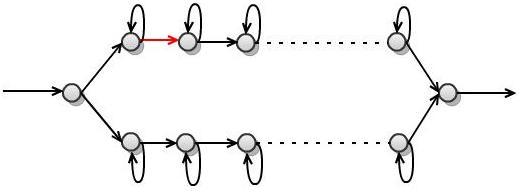
\includegraphics[scale=.75]{valiant1.jpg}
\end{center}              
Observe that a cycle cover for the vertices in this gadget should contain exactly one of the two paths. For the vertices in the other path, the self loops are to be considered in the cover. Note that no cycle cover can choose self loops in both paths and cover the entry and exit nodes. Without loss of generality, assume that the path above corresponds to the variable being 1 and the one below corresponds to the variable being 0.  Connect all the variables in the expression in a loop.
            \item
                There is a clause gadget corresponding to each clause in the expression.
              \begin{center}  
                 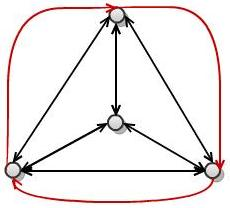
\includegraphics[scale=.75]{clause.jpg}
                 \end{center}
Observe that, to cover all four vertices, at least one of the three outer edges coloured in red must be left out. Associate each outer edge to a variable in the clause and assume that the edge is not chosen in the cover if the corresponding variable is 1. This ensures that every clause has atleast one variable that is 1 and hence the existence of cycle cover implies the existence of a satisfying assignment to the expression.
            \item
                To ensure that the value of the variable is consistent between the variable and clause gadgets, introduce a connector gadget as shown below.
                \begin{center}
                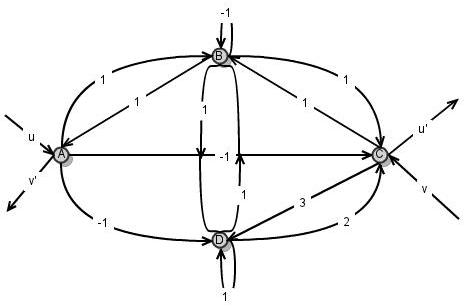
\includegraphics[scale=.75]{connector.jpg}
                \end{center}
                In the clause gadget, the outer edge corresponding to a variable is removed and the above gadget is introduced so that the vertices adjacent to the removed edge in the clause gadget are connected at $u$ and $u'$. Similarly, in the variable gadget, one edge from the top path, say the edge coloured in red, is removed and this gadget substituted in its place so that the vertices adjacent to the removed edge are connected at $v$ and $v'$. The construction of the connector is such that both $u$ to $u'$ and $v$ to $v'$ would not be in the cycle cover simultaneously. This ensures the consistency of a variable value between the two gadgets.
        \end{enumerate}
        To show that $\#CC(G)=\#\SAT(\phi)$, we have to verify if the connector gadget allows only paths $u$ to $u'$ or $v$ to $v'$ to contribute to the cycle cover and that the connector gadget doesn't contribute to the cycle cover if neither of the paths is chosen. Consider the following cases and the corresponding ways for vertices to be a part of cycle cover and the corresponding contribution to the final sum:
        \begin{enumerate}
            \item
                None of $u$, $u'$, $v$ or $v'$ is used. 
                \begin{enumerate}
                    \item (AB)(DC) contributes 6 
                    \item (ADCB) contributes -2
                    \item (ACB)(D)  contributes  -1
                    \item (ACDB)  contributes    -3
                \end{enumerate}
                Net contribution = 0.
            \item
                Cover passes from $u$ to $v'$. $v$ and $u'$ are not used.                 \begin{enumerate}
                    \item (BC)(D) contributes 1 
                    \item (CD)(B) contributes -6
                    \item (BCD)  contributes  3
                    \item (BDC)  contributes  2
                \end{enumerate}
                Net contribution = 0.
            \item
                Cover passes from $v$ to $u'$. $v'$ and $u$ are not used.                 \begin{enumerate}
                    \item (AB)(D) contributes 1 
                    \item (ADB) contributes -1
                \end{enumerate}
                Net contribution = 0.
            \item
                Cover passes from $u$ to $v'$ and also $v$ to $u'$.                 \begin{enumerate}
                    \item (BD) contributes 1 
                    \item (D)(B) contributes -1
                \end{enumerate}
                Net contribution = 0.
            \item
                Cover passes from $v$ to $v'$ and hence $u$ and $u'$ not used.           \begin{enumerate}
                    \item (CDBA) contributes 3 
                    \item (CBA) contributes 1
                \end{enumerate}
                Net contribution = 4.
            \item
                Cover passes from $u$ to $u'$ and hence $v$ and $v'$ not used.           \begin{enumerate}
                    \item (ABC)(D) contributes 1 
                    \item (AC)(BD) contributes -1 
                    \item (AC)(B)(D) contributes 1 
                    \item (ADC)(B) contributes 2 
                    \item (ADBC) contributes -1 
                    \item (ABDC) contributes 2 
                \end{enumerate}
                Net contribution = 4.
        \end{enumerate}
        Observe that, for every variable in the clause, there is a contribution of $4$ to the solution of \#$CC$. Therefore, \#$CC(G) = 4^{3m}\#\SAT(\phi)$ as there are $3m$ connector gadgets in total in the graph ($m$ clauses in the 3-CNF). Thus, \#\SAT is reduced to \#$CC$ which is equal to \perm($A$). However, in this argument, the matrix is over $\{-1, 0, 1, 2, 3\}$. The problem of computing permanent of an integer matrix can be reduced to the problem of permanent computation of $(0,1)$-matrix as follows. %For an integer matrix $A$, such an $(0,1)$-matrix $B$ is found by the following steps.
        
        \begin{remark}
        We remark that the above reduction gives the following observation : for a given graph is the sum of weights of cycle covers is positive is as hard as $\SAT$.
        \end{remark}
    \begin{enumerate}
        \item 
            {\bf Reduction from integer matrix to non-negative integer matrix}: Let A be an $n \times n$ integer matrix in which no entry is larger than $\mu$ in magnitude. From the definition of the permanent, it follows that $|\perm(A)| \leq n!\mu^n$. To compute $\perm(A)$
            it is sufficient to compute its value $\mod Q$ for $Q > 2n!\mu^n$. Formally, given $A$ compute $Q = 2n!\mu^n + 1$, $A' = A \mod Q$ and $P = \perm(A') \mod Q$. If $P < Q/2$ then $\perm(A) = P$. Otherwise $\perm(A) = P - Q$ (value is negative). This transformation is done in polynomial time.
        \item 
            {\bf Reduction from non-negative integer matrix to matrix with only non-negative powers of two}: Replace edges as follows: if the weight of the edge is $w$, such that, $w = 2^{x_1} + 2^{x_2}+\dots+2^{x_r}$, replace the edge by the following construct.
            \begin{center}
            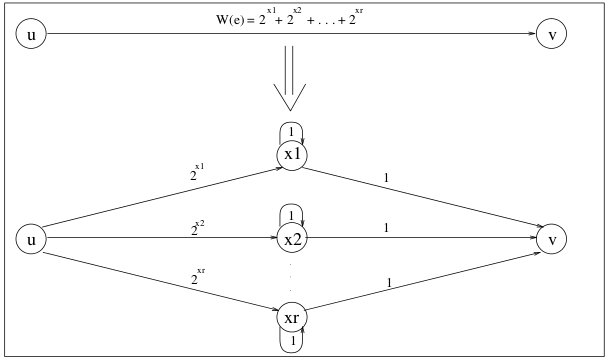
\includegraphics[scale=.6]{reduction1.jpg}
            \end{center}
            This doesn't affect the value of the sum of cycle covers. 
        \item
            {\bf Reduction from  matrix with only non-negative powers of two matrix to a $(0,1)$- matrix}: Replace edges as follows: if the weight of the edge is $2^m$, replace it with the following construct.
                       \begin{center}
            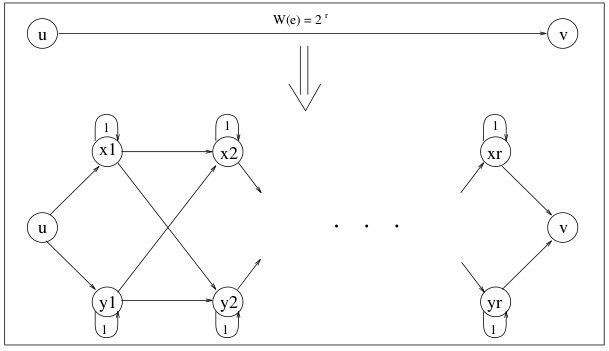
\includegraphics[scale=.6]{reduction2.jpg}
            \end{center}
            Once again, observe that the value of the sum of cycle covers doesn't change and the resultant graph $\in \{ 0, 1\}^{n \times n}$.
    \end{enumerate}
    Thus, for an integer matrix $A$, there exists an $(0,1)$-matrix $B$, such that, $\perm(B) = \perm(A) (\mod Q)$. Hence, from {\bf Lemma 1}, we can conclude that \perm($A$) is \#\P-complete, if A is a $(0,1)$-matrix.
    \end{proof}
        \begin{remark}
		Why does this not contradict the fact that we can efficiently test if $\perm$ is positive for 0-1 matrices. Notice that the $\mod$ does the trick. The value of the permanent will be computed only $\mod Q$. The actual value of the permanent after substitution could be much larger, and we are guaranteed equality only $\mod Q$. Hence a zero value under this computation does not mean that permanent value of the matrix is zero, it just means that it is a multiple of $Q$.
        \end{remark}
\end{document}
